\chapter{心包积液与心包摩擦音}

心包积液与心包摩擦音都是心包疾病的重要体征。心包积液通常可经体格检查与X线检查确定。心包摩擦音则只有经由听诊而作出诊断,但由于其变化不定,往往是出现快而消失也快,在急性炎症病程中天天反复听诊才易于发现。心包摩擦音对干性心包炎有决定性诊断意义。心包积液则可见于渗出性心包炎及其他非炎症性心包病变。

干性心包炎(纤维素性心包炎)以心包摩擦音为临床特征。此音在病程中出现最早,通常也为整个病程中唯一的体征。此音通常在胸骨左缘心前区听到,呈微细的抓搔性质或具有较粗糙的刮擦性质,不向任何方向扩散,也不与心脏活动的某一时期相符合(在收缩期终末时较强,又侵占舒张期的初段)。此音有时只在短期内听到。有些病例触诊可同时发现心包摩擦感。干性心包炎发病可急骤,伴有高热与重度全身不适,但少数发病缓慢渐进,几乎无任何不适,多数病例因心前区痛就诊,可甚严重,须与急性心肌梗死、胸膜炎、自发性气胸或纵隔气肿等相区别,急性心包炎时,胸痛的特点是深呼吸时或转动胸廓时加剧,应注意与急性肺栓塞的胸痛鉴别,急性心肌梗死的胸痛则不具此特点。如胸痛发生后24小时内能听到心包摩擦者,则更支持急性心包炎。心电图检查常有助于二者的鉴别。

渗出性心包炎最常见的症状是气短与胸部郁闷感,有时心前区有持久的压迫性疼痛。如心包内有大量渗出液,可发生严重的呼吸困难,触诊心尖搏动微弱与未能触知,叩诊心浊音界向两侧扩大,呈梯形或三角形,心底部浊音范围卧位时增宽、坐位时缩小,心浊音皆为绝对浊音,听诊在肩胛角下一片浊音区(Ewart征),有时可见心前区胸壁的肋间隙展平,或有轻度皮肤水肿。脉搏细速,动脉血压下降,脉压小,静脉压上升,当积液大量时出现奇脉(吸停脉)。迅速增长的大量心包积液可引起心包压塞征。临床表现为静脉压不断升高、颈静脉怒张、进行性肝大、心动过速、动脉血压持续下降,甚至发生休克。

在心包积液时,X线检查心脏正常轮廓消失,心影呈三角形或梯形扩大,卧位时心底部阴影加宽,立位时缩窄,心搏显著减弱,往往与心底部大血管阴影的正常有力搏动呈鲜明的对比:如积液量少,则叩诊检查不如X线检查的准确。心包积液量甚少时,在病程进行中需重复X线摄片,作前后对比,较易发现心脏阴影增大,而提示渗出性心包炎的诊断。

渗出性心包炎的心电图所见为窦性心动过速,普遍性低电压,胸导联R波电压降低,尤以V\textsubscript{5}
的R<1mV具有较高敏感性,再结合肢体导联电压降低是重要的诊断线索(图\ref{fig17-1})。在疾病的早期,各导联ST段凹面向上抬高(S-T\textsubscript{aVR}
下降)、T波高耸,与心肌梗死的改变不同,故甚有助于与心肌梗死的鉴别诊断(表\ref{tab17-1})。

\begin{figure}[!htbp]
 \centering
 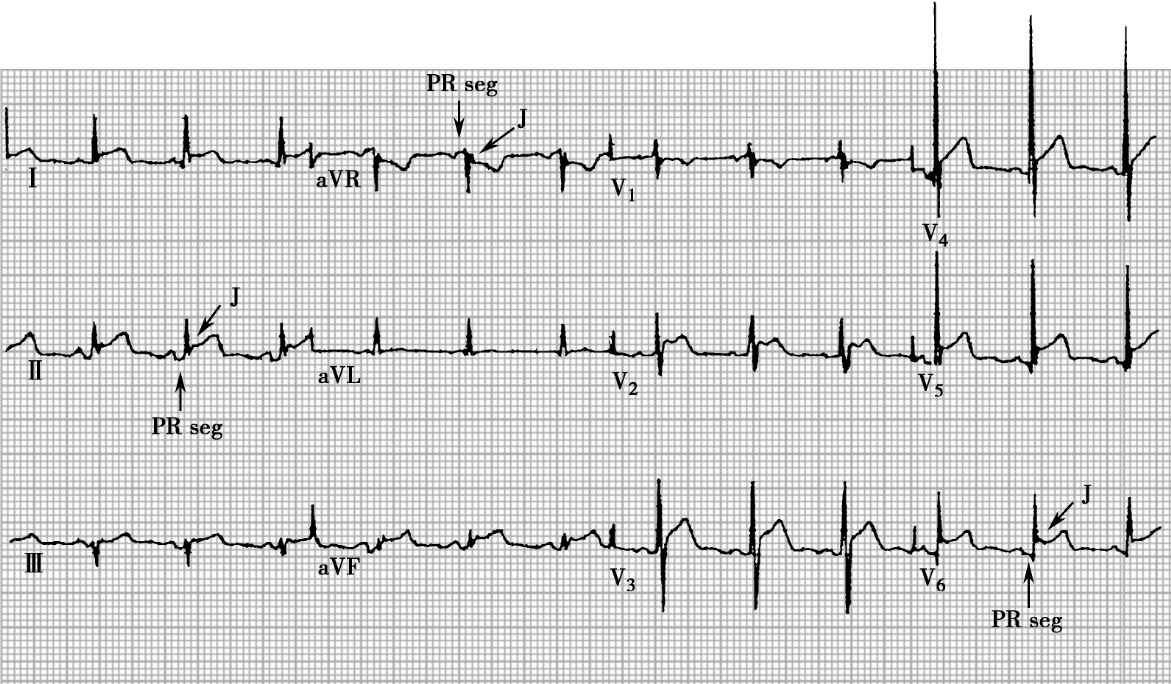
\includegraphics[width=5.40625in,height=3.13542in]{./images/Image00103.jpg}
 \captionsetup{justification=centering}
 \caption{急性心包炎心电图}
 \label{fig17-1}
  \end{figure} 

\begin{table}[htbp]
\centering
\caption{渗出性心包炎心电图表现与急性心肌梗死鉴别}
\label{tab17-1}
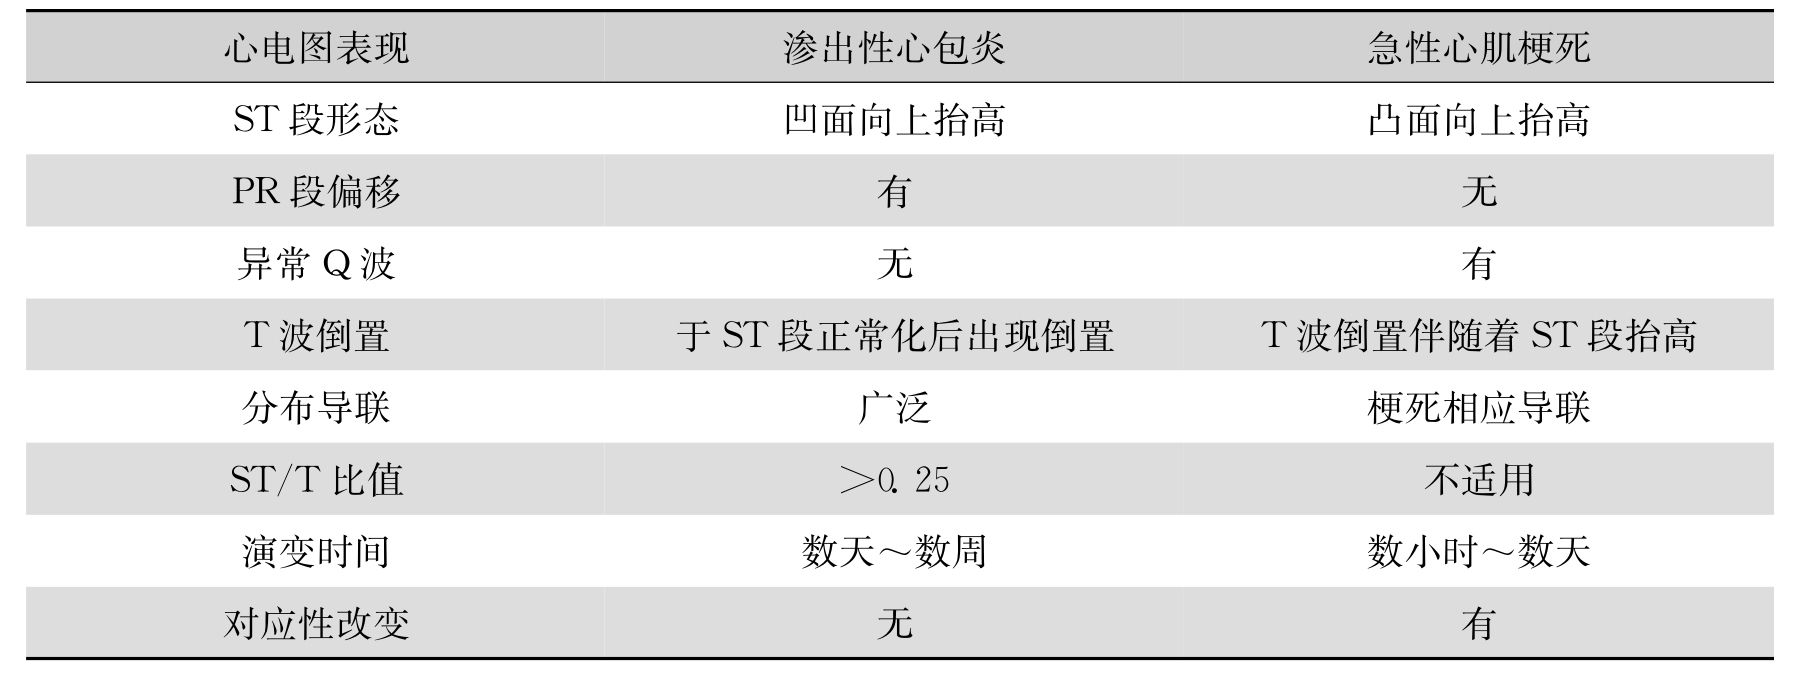
\includegraphics[width=5.97917in,height=2.25in]{./images/Image00104.jpg}
\end{table}

偶尔在个别的心肌疾病(如心肌炎、脚气病性心脏病)病例,由于心脏高度普遍性增大,心影向两侧扩大,并可出现心脏搏动微弱与心音减弱、脉压小等类似渗出性心包炎的征象;又如心肌松弛,卧位时也可出现心底部加宽的改变,致可互相混淆。渗出性心包炎与心脏普遍性增大的鉴别(表\ref{tab17-2}),除根据心脏搏动与心音的强弱、心界随不同体位而改变、奇脉之有无等体征之外,尚需同时参考下列各点:

\begin{longtable}{c}
 \caption{渗出性心包炎与心脏普遍性增大的鉴别}
 \label{tab17-2}
 \endfirsthead
 \caption[]{渗出性心包炎与心脏普遍性增大的鉴别}
 \endhead
 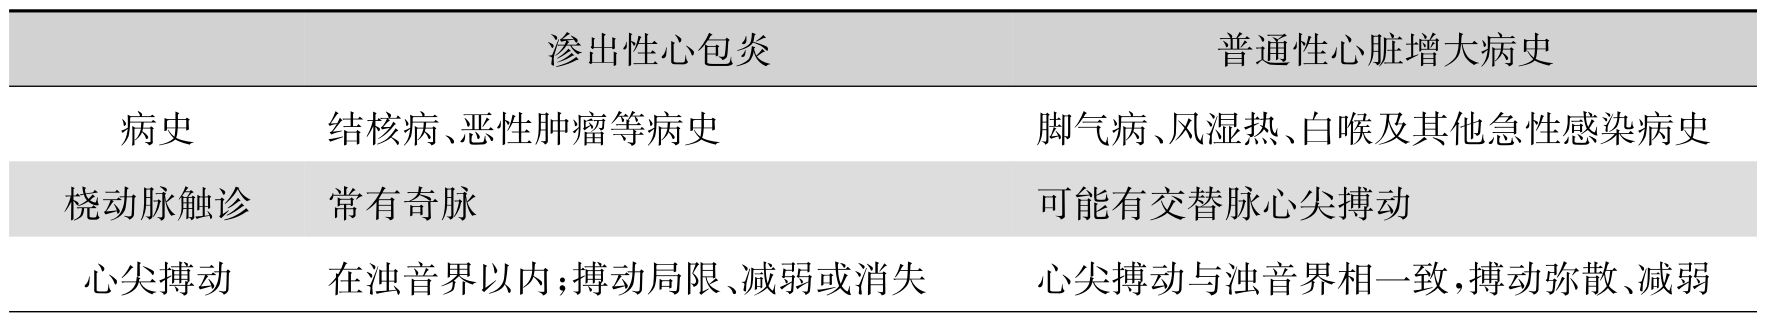
\includegraphics[width=\textwidth,height=\textheight,keepaspectratio]{./images/Image00105.jpg}\\
 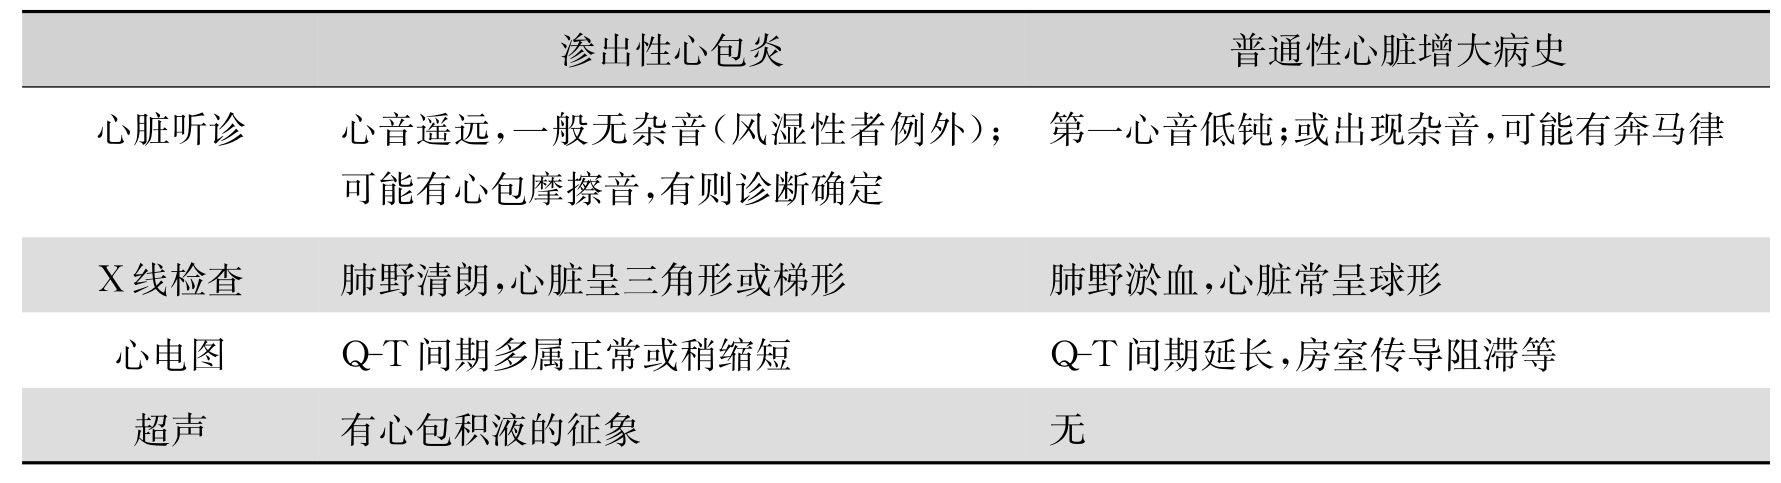
\includegraphics[width=\textwidth,height=\textheight,keepaspectratio]{./images/Image00106.jpg}
 \end{longtable}

\section{(1)心脏听诊:}

如先有心包摩擦音出现,则渗出性心包炎的诊断确定。

\section{(2)胸部透视:}

渗出性心包炎时肺野在X线透视下常较清朗,而心脏增大时则常合并肺淤血。

\section{(3)心脏右前斜位透视:}

在食管吞钡检查时,渗出性心包炎与心脏增大虽都可将食管压向后方,但二者的表现不同:前者将食管后压成一较大的弧形,位较靠下;后者多伴有左右两侧心力衰竭,由于左右心房扩大的结果,致将食管向后压迫,可形成两个弧形。

\section{(4)心电图检查:}

在渗出性心包炎时Q-T间期仍为正常,而心脏增大时Q-T间期常显著延长。

\section{(5)X线记波摄片:}

根据波形的改变,有助于诊断和鉴别心肌疾病与心包疾病(心包粘连、心包积液)。近年来有医院行心包充气造影,比常规心脏摄片更好的显示心包腔,壁层心包厚度、形态及心脏影,在诊断心包钙化、心包缩窄方面有较高的敏感性。

\section{(6)超声检查:}

对提示心包积液的有无、多少与穿刺定位,往往有重要的帮助,心包压塞时超声心电图有特征性表现。二维超声心动图目前是区别全心包积液和包裹性心包积液的金标准。

\section{(7)血流动力学检查:}

对心包压塞与慢性缩窄性心包炎的诊断和鉴别诊断有一定的价值。

\section{(8)CT扫描:}

多层次断面摄影能清晰观察心包病变。CT扫描能根据心包增厚、粘连和钙化,而作出缩窄性心包炎的诊断。

\section{(9)诊断性心包穿刺:}

如上述检查未能明确病因学诊断,则在B超导引下作心包诊断性穿刺,抽取积液作病因学检查。

\section{(10)纤维心包镜检查:}

现普遍采用导管和心包穿刺相结合的方法,可以提供心脏压塞绝对肯定的诊断,测定血流动力学的受损情况,通过心包抽液血流动力学改善的证据来指导心包穿刺抽液,可以测定同时并存的血流动力学异常,已成为心包疾病的重要诊断手法之一。

引起心包积液与心包摩擦音的疾病颇多,现按表\ref{tab17-3}的顺序讨论于下:

\begin{longtable}{c}
 \caption{引起心包积液与心包摩擦音的疾病分类}
 \label{tab17-3}
 \endfirsthead
 \caption[]{引起心包积液与心包摩擦音的疾病分类}
 \endhead
 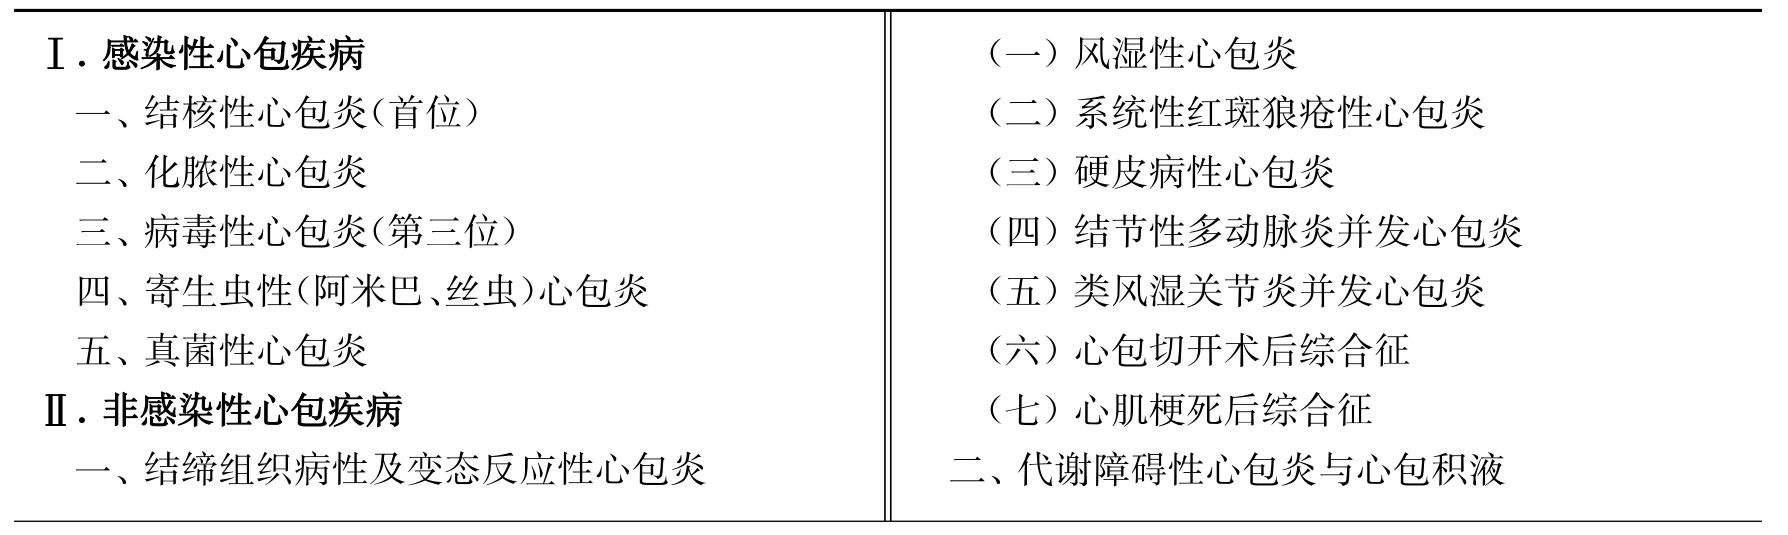
\includegraphics[width=\textwidth,height=\textheight,keepaspectratio]{./images/Image00107.jpg}\\
 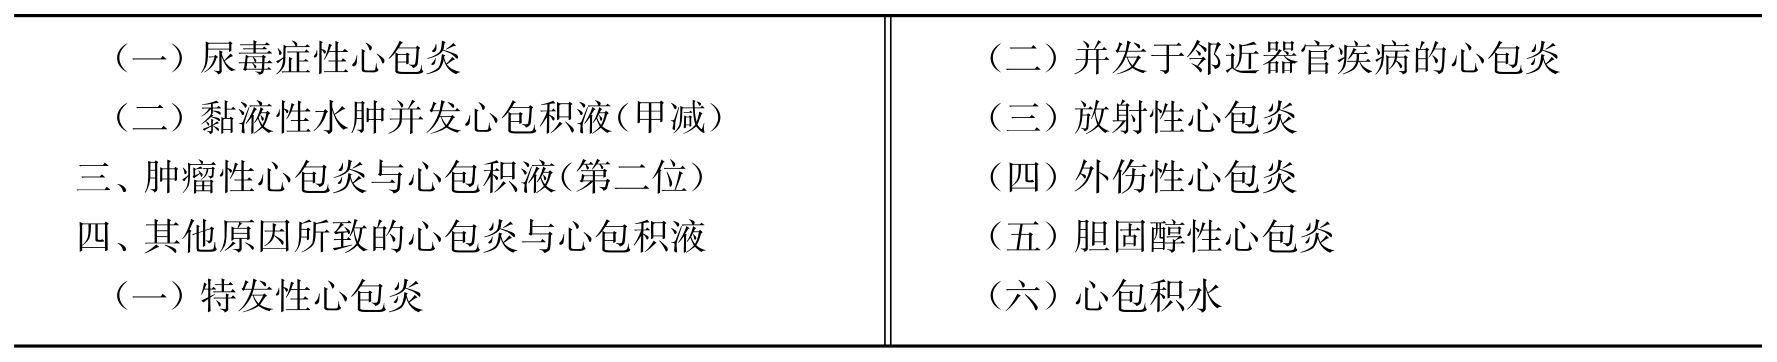
\includegraphics[width=\textwidth,height=\textheight,keepaspectratio]{./images/Image00108.jpg}
 \end{longtable}

\protect\hypertarget{text00145.html}{}{}

\section{54 感染性心包疾病}

\subsection{一、结核性心包炎}

长期发热、心前区疼痛与气促,是结核性心包炎患者就诊时最常见的主诉。此病是较常见的心包疾病,而在各种心包炎中也占最多数,如国内报告一组106例急性心包炎中,结核性占66例。结核性心包炎的临床特点是发病较缓,毒血症症状较轻,渗出液多为大量,且多为血性,病程经过较长,最后常发展为慢性缩窄性心包炎(参见第92节)。

临床上诊断结核性心包炎的主要根据是:①长期不规则的发热,发热虽可较高,但患者往往无严重的中毒面容;②有心包外结核病存在,最常见者为肺结核、结核性胸膜炎与淋巴结结核;③心包渗出液常为大量,可达1000ml或更多,多数为血性,虽经多次抽液,仍有重行积聚的倾向;④血象白细胞总数多为正常,也有轻度增多或轻度减少;⑤心包渗出液培养或动物接种可发现结核杆菌(阳性率为25\%~50\%)。若在渗出早期同时进行心包液和心包活检可见结核性肉芽肿及干酪样坏死灶,确诊的可能性非常大,但必须强调心包活检正常不能排除结核性心包炎,找到肉芽肿及干酪样物质但无活的结核菌也不能诊断;⑥心包液中ADA活性达40U/L或更高的诊断敏感性和特异性分别为93\%和97\%;⑦ELISA检测抗结核抗体(抗PPD-IgG)诊断敏感性和特异性分别为86\%和97.8\%,浆膜腔积液浓度/血液浓度>1支持诊断。结核性心包炎首先需注意与风湿性心包炎相区别(表\ref{tab17-4})。

\begin{table}[htbp]
\centering
\caption{结核性心包炎与风湿性心包炎的鉴别}
\label{tab17-4}

\includegraphics[width=5.98958in,height=2.95833in]{./images/Image00109.jpg}
\end{table}

结核性心包炎的经过轻重不等,有些患者无明显的心包外结核病(例如经常规X线检查未能发现的纵隔淋巴结结核)、发热较低、发热期较短、心包积液细菌学检查阴性、病程较短,与特发性心包炎难以区别,其鉴别见第55.4节。

肝大是结核性心包炎最常见而突出的体征之一,并常伴有疼痛与压痛,同时患者又有长期发热,可被误诊为肝脓肿或胆道感染。

\subsection{二、化脓性心包炎}

化脓性心包炎是经过急重、预后较差的疾病,持续仅数天,只有早期诊断与积极治疗,方有治愈的希望。常见症状有高热、寒战、盗汗、呼吸困难,大部分患者无典型的心包性胸痛症状,几乎所有的患者都有心动过速,但存在心包摩擦音的患者少于半数。化脓性心包炎较多通过以下几个途径而来:①胸腔手术或创伤后早期术后感染的直接蔓延;②与感染性心内膜炎有关;③膈下化脓性病灶蔓延;④菌血症时血行播散。致病菌最多为金黄色葡萄球菌,其次为大肠杆菌、肺炎双球菌、链球菌等,化脓性心包炎常继发于化脓性皮肤感染、败血症、肺炎、骨髓炎等病程中。但也有不少未查出原发病灶,心包渗出液为脓性或脓血性,常能找到化脓性细菌。肺炎并发心包炎在发病初期最易忽略,如能发现心包摩擦音,则可确定诊断。心包积液培养在病原学诊断上有重要意义。

概括说来,化脓性心包炎的诊断依据有:①急性感染全身中毒症状严重,如高热、白细胞增高等;②有急性心包填塞的症状;③ECG示低电压,ST段和T波改变;④X线片显示心影扩大;⑤心包穿刺获脓液可确诊;⑥B超见心包增厚,心包内液性暗区,特别是心包内探及光点增粗的絮状物诊断价值更大。

误诊或漏诊的原因可能由于:①原发性化脓感染灶或败血症的临床表现比较突出,以致对心包炎的体征未及注意而致漏诊;②起病较缓,一般中毒症状不太严重,血象白细胞计数不太高,或由于病初心包积液中未见有大量脓细胞,或由于心包积液为血性,致误认为结核性心包炎。一旦怀疑或确诊化脓性心包炎应立即行心包穿刺,查心包积液的革兰氏、抗酸染色与真菌,并做心包积液与体液培养。

有报道肺胸膜放线菌病可蔓延至心包膜而引起心包炎。

\subsection{三、病毒性心包炎}

临床上大多数非特异性心包炎极可能为病毒所致,已确诊为乙组柯萨奇病毒、埃可病毒、乙肝病毒所致的心包炎,国内仅见少数报道。带状疱疹病毒致急性心包炎国内见一例报道。病变可累及心肌与心包。此病主要流行于夏、秋二季,但也可为散发性。病情较轻,病程短。心包积液及(或)心包组织检查是确诊的必要条件,主要依据PCR或原位杂交技术,血清抗体滴度增加4倍可提示但不能确诊。柯萨奇病毒可从患者粪便与鼻咽部分泌物中分离出,也有助于此病的诊断。

\subsection{四、寄生虫性心包炎}

\subsubsection{(一)阿米巴性心包炎}

阿米巴性心包炎临床上罕见,常见阿米巴肝脓肿向心包腔穿破引起。患者有一般急性心包炎的症状与体征。如患者有肝脓肿或(及)胸膜阿米巴病而出现心包病征,应考虑本病,心包穿刺可抽得棕褐色(巧克力色)脓液,是此病的特点。但在心包穿刺液涂片中不易找到溶组织阿米巴滋养体,而培养则较易于发现。如作抗阿米巴治疗(氯喹、甲硝唑)获得治愈,可证实诊断。后期可演变为慢性缩窄性心包炎。

\subsubsection{(二)丝虫性乳糜性心包炎}

此病罕见,国内仅有少数病例报告。大多数患者无胸痛、胸闷等明显症状,常于X线片或超声心动图上发现大量积聚缓慢的心包积液时引起注意。心包积液为乳糜性,镜检微丝蚴阳性,血中微丝蚴也呈阳性,经穿刺抽液与乙胺嗪、卡巴胂治疗后心包积液完全吸收,血中微丝蚴也消失。

\subsection{五、真菌性心包炎}

国外文献也有报道荚膜组织胞浆菌引起的心包炎。此病的好发人群包括免疫功能低下(先天免疫缺陷、使用免疫抑制剂或非甾体类抗炎药、艾滋病等)患者,严重烧伤患者,接受强力广谱抗生素治疗的患者,过度劳累个体以及婴儿(尤其是早产儿)。对原因未明的持久性心包炎,需考虑真菌感染的可能性。

\subsection{六、立克次体性心包炎}

此病罕见,恙虫病(由恙虫病东方立克次体引起的急性传染病)引起的心脏损害主要是心肌炎,少数病例在心脏B超检查出少量心包积液。临床表现以心肌炎所致的心悸、胸闷、胸痛为主,伴高热、皮疹、焦痂、淋巴结肿大,心电图和心肌酶谱有心脏损害的表现,血清外斐反应OXK效价明显增高,诊断不难。氯霉素和强力霉素治疗有效。

\protect\hypertarget{text00146.html}{}{}

\section{55 非感染性心包疾病}

\subsection{55.1 结缔组织病性及变态反应性心包炎}

\subsubsection{一、风湿性心包炎}

据国内临床资料,风湿热合并心包炎者占6\%~12.1\%不等。临床上诊断为风湿性心包炎者为数较少,其原因之一可能为诊断心包炎的重要体征------心包摩擦音持续时间极为短暂(数小时至两三天),易于忽略。

风湿性心包炎多发生于青年人,中年人少见,而老年人则更少见,单纯的风湿性心包炎少见,患者常合并风湿性心肌炎与心内膜炎,即所谓全心炎,且心肌炎与心内膜炎的征象常较突出。风湿性心包炎与常与心脏外风湿性病变并发,最多者为多发性关节炎。

风湿性心包炎可为干性(纤维素性)或渗出性(浆液纤维素性)。在风湿病过程中出现心包炎时,提示风湿病的活动性加重,临床上出现体温突然升高、血沉加快、心搏与呼吸显著加速。此种心搏与呼吸次数的增加,往往超过体温升高时常见的比例。心包摩擦音常仅持续短暂时间而消失,或时隐时现,因此临床上可能忽略;临床上对拟诊为风湿热的患者,当病情加重时,须天天注意细心听诊,方可有所发现。

风湿性心包炎的诊断标准依据如下:有心前区胸痛、心包摩擦音或有心包渗出的超声心动图的证据,同时具有关于急性风湿热的临床标准和原先的A组链球菌感染血清学证据。

风湿性渗出性心包炎通常为浆液性,极少为血性,液量通常不多,一般不超过300ml,但偶尔也可多至1000ml或以上,如渗出液量较少,通常经2~3周自行吸收,因而甚少需作心包穿刺抽液,水杨酸制剂及肾上腺皮质激素对此病有优良的疗效。

风湿性心包炎痊愈后,一般只引起局限性松弛的粘连,不累及整个心包,因此不致妨碍心脏活动功能。国内仅见1例报道风湿性心脏病二尖瓣狭窄合并原因不明的缩窄性心包炎。

风湿性心包炎与结核性心包炎的鉴别诊断,主要根据患者风湿热的其他表现、发病较急、病程较短,以及对水杨酸制剂的优良疗效和较良好的预后,其与特发性心包炎的鉴别参见第55.4节。

\subsubsection{二、系统性红斑狼疮性心包炎}

系统性红斑狼疮性心包炎常在活动期突然发生,但也可发生于亚急性期或慢性期。心包炎的存在国内临床报道约1/4出现明显症状体征。心包炎多数为干性,主要体征为心包摩擦音,痊愈后常遗留心包粘连增厚,如发生心包积液,多为浆液纤维素性,少数为血性,积液可达数百毫升,细胞分类以中性粒细胞为主。在周围血液内或(及)心包渗出液内找到狼疮细胞,抗核抗体阳性可确定此病的诊断。

此病在鉴别诊断上须注意与风湿性及结核性心包炎相区别。患者常有游走性关节痛、发热、血沉加快、心电图上甚或可出现P-R间期延长,肾上腺皮质激素治疗有显著疗效,与风湿性心包炎相似,但根据患者的特征性面部蝶形红斑、白细胞减少、肾脏损害的表现等,应多考虑系统性红斑狼疮的可能性,有决定性意义的是面部蝶形红斑及红斑狼疮细胞的发现。如临床表现符合,两项征象当中出现任何一项时,即可肯定诊断。此病与结核性心包炎的鉴别,除根据后者常有心脏外结核病、积液通常为大量、积液中可找到结核杆菌,一般无显著的白细胞减少等情况外,主要仍根据本病有多个器官损害的征象,面部蝶形红斑或(及)狼疮细胞的发现,血清抗核抗体效价升高等。

\subsubsection{三、硬皮病性心包炎}

硬皮病心脏受累常为晚期征象。由此病引起的心包炎十分罕见。心包积液的特征是草绿色,蛋白含量>5g/L,细胞数量少,无自身抗体,补体和免疫复合物含量低。

\subsubsection{四、结节性多动脉炎并发心包炎}

结节性多动脉炎甚少并发心包炎,偶尔引起大量血性心包积液并出现心包压塞症状。

\subsubsection{五、类风湿关节炎并发心包炎}

近年强调类风湿关节炎可为成人心包炎病因之一。但也可见于儿童乃至60岁以上的类风湿关节炎病例。其常见表现为发热、心前区疼痛、呼吸困难和心包摩擦音,并伴有关节炎症加重和胸膜炎。结缔组织病的心脏表现与心包炎发生率见表\ref{tab17-5}。

\begin{table}[htbp]
\centering
\caption{结缔组织病的心脏表现}
\label{tab17-5}
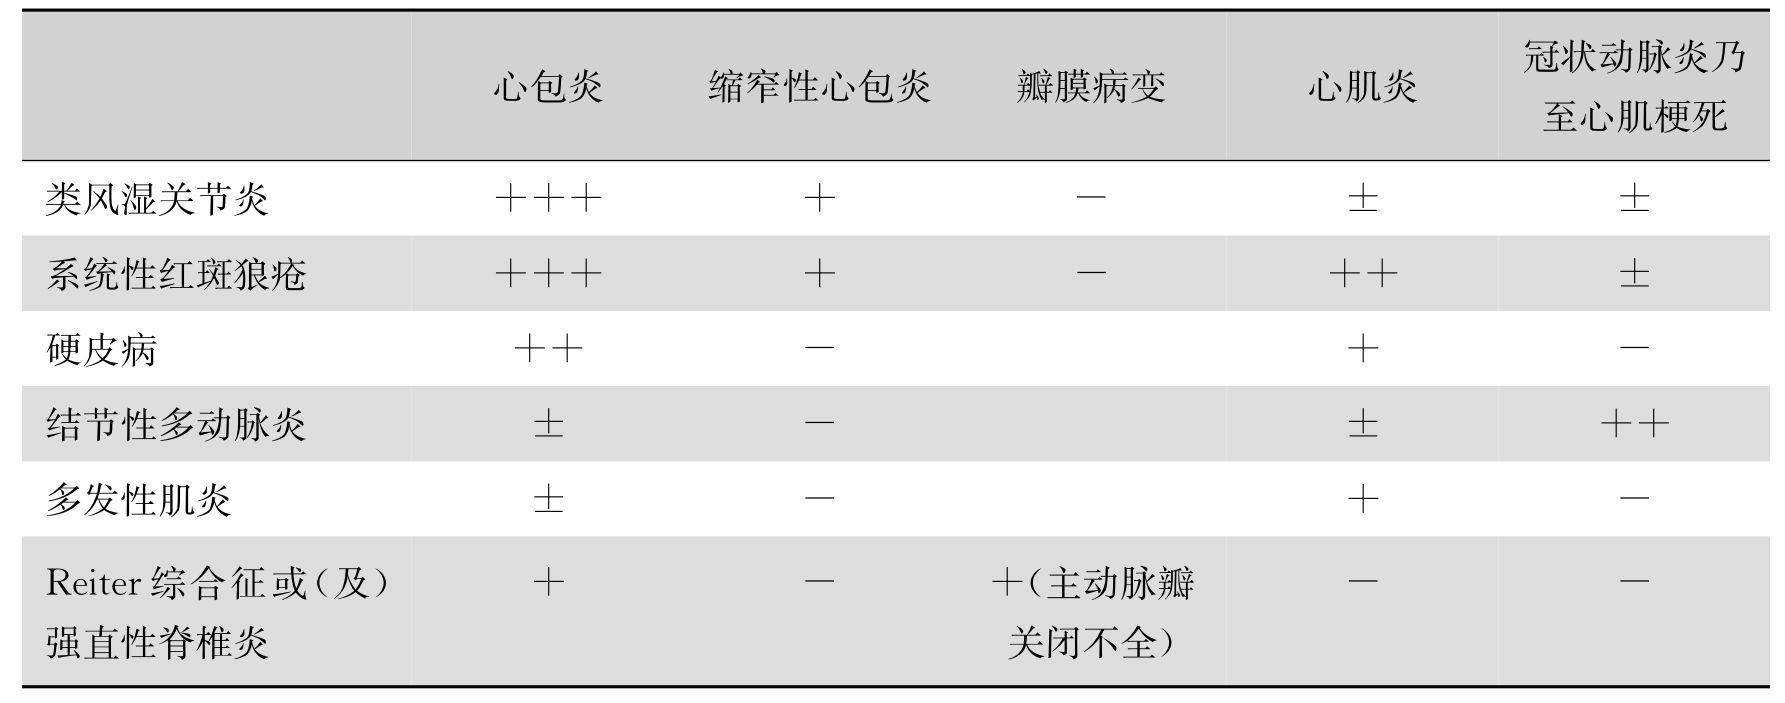
\includegraphics[width=5.9375in,height=2.33333in]{./images/Image00110.jpg}
\end{table}

\subsubsection{六、白塞病性心包炎}

白塞病伴有较高的心脏病变发生率,急性心包炎是其最常见的心脏损害。心包积液可以是纤维蛋白性或渗出性,也可合并胸腔积液,结合其特征:反复发作的口腔溃疡、生殖器溃疡、眼色素膜炎、皮肤损害等,诊断不难。国内报告一组42例有心脏损害的白塞病,其中10例表现为心包积液,糖皮质激素或免疫抑制剂治疗有效。

\subsubsection{七、心包切开术后综合征}

在心脏手术(如先天性心脏病手术、二尖瓣分离术)后10天至4周间,患者可出现发热、胸痛、心包炎、胸膜炎等症状,症状轻重不一。实验室检查有白细胞增多、血沉加快、嗜酸性粒细胞暂时性增多、C反应性蛋白试验阳性等改变。50\%病例有心包摩擦音,有些病例则出现不同程度的心包积液,积液可以是草绿色的、血清样的或纯血性的,蛋白含量高于4.5g/dl,白细胞计数在3000~8000/mm\textsuperscript{3}
(包括淋巴细胞和粒细胞)。心包积液与胸腔积液均未能证明有细菌的存在。症状常能自行缓解。必须注意的是心包积液在心脏手术后是非常普遍的,在术后10天内有56\%~84\%的患者发生。所以,心包切开后综合征的诊断必须排除其他原因引起的术后发热,包括感染和病毒诱发的灌注后综合征,后者具有不典型的淋巴细胞增多、发热及脾大。本病预后优良。发病机制可能与自身免疫作用有关。

\subsubsection{八、心肌梗死后综合征}

也称Dressler综合征,其发病机制有人认为可能与自身免疫有关。病情经过良好,典型病例发生于心肌梗死之后1周至数月,发生率为0.5\%~5\%。主要临床表现有持续发热、胸痛、血沉加快、白细胞增多、心包炎、胸膜炎与肺炎等。此综合征主要与继发于急性心肌梗死的心包炎相区别:后者心包摩擦音发生较早,通常在心肌梗死后第2~4天出现,持续时间短而易于消失,一般不产生明显的心包积液,心电图特征是P-Q段持续压低超过24小时;此综合征心包摩擦音出现较晚(大约在心肌梗死后第2~11周),持续较久(7~10天或数周),有时并发左侧胸腔积液,有些病例有心包积液,甚至需要穿刺放液,因此二者一般不难区别。不伴有心脏压迫的心梗后心包炎必须与急性肺栓塞,更重要的是与反复心肌缺血相鉴别:①硝酸甘油可明显缓解疼痛;②无心包摩擦音;③新出现的区域性ST段和T波改变伴有相对应的改变,为反复心肌缺血的特征表现;④心梗后心包炎典型的T波形态演变特征:心梗发病数天后ST段恢复至基线伴T波低平、倒置,数周或数月后T波恢复正常。

\subsubsection{九、其 他}

国内报道一例亚急性甲状腺炎(De
Quervain病)致心包积液,为中量稀薄渗出液,激素治疗有效。

\subsection{55.2 代谢障碍性心包炎与心包积液}

\subsubsection{一、尿毒症性心包炎}

尿毒症性心包炎是一种伴有纤维素性渗出物的无菌性炎症,常发生于慢性肾衰患者透析之前或透析开始数月中。国内文献报告尿毒症患者12.9\%~35\%合并尿毒症性心包炎,一般认为由于体内氮代谢产物与酸类蓄积,刺激心包膜而引起。通常少有渗出液,主要体征为心包摩擦音,出现于心底部、心前区或局限于狭小的区域。患者常有不同程度的心前区疼痛或仅有压迫感,但不一定有发热。由于患者的尿毒症症状相当明显,心包炎本身的症状往往较不显著。

尿毒症性心包摩擦音往往为尿毒症后期的表现。但如尿毒症的原因为可逆性,则一旦肾功能改善后,心包摩擦音常可消失。

慢性肾衰竭患者做慢性透析时,可于透析开始后不久出现心包炎,发生原因与尿毒症及肝素化引起渗血有关,也可同时并发心肌病变,表现为奔马律、心律失常等。

\subsubsection{二、黏液性水肿并发心包积液}

黏液性水肿并发心包积液者近年来有增多的趋势,其原因以甲状腺功能减退为主,甲状腺功能减退的患者5\%~30\%可发生心包积液。患者有黏液性水肿的一般表现,心包积液征象,并且可有巨舌及静脉压升高,这些表现均为甲减的特征。婴儿、老年人患者可能无症状。有时需与结核性心包炎相区别。其特征是心包积液量很大,心率不快,心包压塞症状不明显,积液比重高、富含蛋白质与胆固醇,而细胞数少,应用甲状腺制剂治疗,症状迅速好转。

\subsection{55.3 肿瘤性心包炎与心包积液}

心包肿瘤往往为继发性,原发肿瘤通常为肺癌、乳腺癌、淋巴瘤、白血病及腹腔脏器肿瘤等,但身体任何部位的癌,均可转移至心包。心包原发肿瘤有间皮瘤、畸胎瘤、血管肉瘤、恶性组织细胞病等,均很少见。心包积液常为血性,可为大量,虽经反复穿刺抽液仍再次渗聚。如患者年龄较大,且体内有原发癌,发病徐缓隐袭,心前区疼痛轻微或不明显,积液为血性,应多考虑心包转移癌的可能性。也见一例淋巴瘤纵隔受累引起乳糜性心包积液的报道。如在心包积液中找到癌细胞,则诊断明确,癌性心包炎近年国内报告有增加的趋势,主要见于老年人。还应注意的是2/3恶性心包积液患者积液原因是放疗,而非肿瘤所致,故应做心包穿刺液检查。

有些病例由于癌组织崩溃或混合感染而致发热。如原发癌隐蔽,则须注意与结核性心包炎相区别。晚期肿瘤患者由于恶性疾病本身或接受治疗使免疫受抑制,亦有可能合并结核性或真菌性心包炎。

白血病性心包炎少见,一般见于急性白血病。此病的诊断一般不难,如白血病患者有心包炎的表现,而能除外其他原因者,一般都可诊断为白血病性心包炎,心包积液大多为浆液血性,不白血性白血病的白血病性心包炎诊断较为困难,由于此时血象无明显改变,易被误诊为结核性心包炎或播散性红斑狼疮心包炎。另一方面,偶尔结核性心包炎也可引起类白血病反应,与白血病性心包炎相混淆,但此反应在积极的抗结核疗程中一般持续时间不长,经动态观察可以鉴别。蒽环类化疗药物阿霉素等的心脏毒性亦可表现为心包炎,应注意鉴别。偶尔恶性组织细胞病以心包炎为主要临床表现,但骨髓涂片检查可确定诊断。

\subsection{55.4 其他原因所致的心包炎或心包积液}

\subsubsection{一、特发性心包炎}

急性特发性心包炎又称急性非特异性心包炎,是近几十年来急性心包炎的主要病因之一,病因不明,可能与病毒感染及其引起的免疫反应有关,目前有许多学者将此病和病毒性心包炎归为一类。

其诊断依据概括是:①发病前约2/3有急性病毒感染史;②起病急骤,高热,剧烈胸痛;③有心包摩擦音;④心包穿刺为非特异性浆液;⑤病程短(4~8周)。约三分之二患者于发病前数周曾患急性上呼吸道感染,急性期与恢复期血清病毒抗体效价可有改变,提示病因可能为病毒。

急性非特异性心包炎在病理学上为一种浆液纤维素性心包炎,多见于青壮年人,经过一般良好,但有复发倾向为其特征。此病的临床特点是多数发病急骤,伴有剧烈的胸骨后或心前区疼痛、发热、心包摩擦音,以及小量乃至中等量心包渗出液,但也见有大量积液引起心包压塞者。血象常呈轻度或中等度白细胞增多。心前区痛为最突出的症状,几乎见于所有的病例。疼痛性质为刺痛、刀割样痛、绞痛或重压感等,呈阵发性或持续性。疼痛可向肩部、背部及手臂放射。常有发热,多属轻度,但也可高达40℃。发热可持续数天乃至3~6周之久。约23\%病例有再发,国内报告一组3例反复发作的原因未明的心包炎,一例病程长达222天,一例并发渗出性胸膜炎,各例均有明显的心包压塞征象,但经ACTH静脉滴注治疗后很快改善。

此病最重要的体征是心包摩擦音,发生率在70\%以上;如注意及早检查,则大多数病例都可发现,通常在胸痛发生后数小时即可听到,多在24~48小时后消失,但也有持续数周或数月之久的,少数病例可出现奔马律,偶有发生阵发性心动过速,约25\%病例伴发胸腔渗出液。心包积液为浆液性,呈草黄色、暗黄色、琥珀色,也可为血性,细菌检查阴性。后期不致发展为缩窄性心包炎。

此病与其他原因所致的急性心包炎鉴别,通常多无困难。

风湿性心包炎发病虽急,但发热往往较高,心前区疼痛轻微,临床上大多同时伴有心肌炎、心内膜炎、多发性关节炎或其他风湿热病征,心电图描记可发现P-R间期延长,水杨酸制剂疗效良好也有助于鉴别。

结核性心包炎进展较慢,胸痛较轻,病程较长,心包积液较多,心包积液可找到结核杆菌,且发展为慢性缩窄性心包炎者甚为常见。二者的鉴别有时并不容易,因此,对于不典型病例,不经过详细的检查与长期观察,不可轻易下急性非特异心包炎的诊断。如结核菌素皮内试验阴性,则结核性心包炎的可能性甚少。对高度怀疑结核性的病例,可考虑进行抗结核治疗,以免耽误病情。

此病也常须与急性心肌梗死相鉴别。

慢性特发性渗出性心包炎少见,病因未明。心包积液持续时间长,患者无明显急性心包炎史,可无心包压塞征象,多数系偶然发现。少数病例最后可发展为心包缩窄。国内作者报道认为早期手术治疗可较晚期行缩窄剥离手术安全和有效。

\subsubsection{二、并发于邻近器官疾病的心包炎}

心、肺、胸膜与纵隔疾病累及心包,引起心包炎者比较少见,急性胰腺炎并发心包压塞亦仅见个案。如心肌梗死的损害由心室肌蔓延至表面,累及心包膜,则可引起浆液纤维素性心包炎,此即继发于急性心肌梗死的心包炎。其主要临床特征为心包摩擦音,通常在心肌梗死发病数天后可听到,有时在患者已无早期病程中的心前区疼痛时,方出现心包摩擦音。此音甚少在发病36小时之内听到,这种情况与急性非特异性心包炎的临床鉴别有重要意义。这种心包炎罕有发生积液现象。在出现心包摩擦音的同时,患者常有发热、白细胞增多、血沉加快等症状,其原因并非由于心包炎症,乃因心肌梗死所致的异性蛋白吸收所引起。继发于心肌梗死的心包炎与心肌梗死后综合征的鉴别参见第55.1节。

主动脉夹层分离患者可因急性心包积血引起心包压塞症状,死亡率高。

\subsubsection{三、放射性心包炎}

纵隔X线放射治疗后可引起放射性心包炎,有时可引起心包缩窄。在放射治疗后须经一段潜伏期(可长达4~6周)然后发病。可并发或不并发放射性肺炎。

国内作者报道放射性心包病有增多的趋势。胸部疾病放射治疗后常引起心包反应。发生率取决于照射部位和剂量的大小。即刻反应(数小时至数月)则引起急性心包炎。延迟反应(数月至数年)则可引起慢性干性心包炎、心包积液、心包缩窄等,迟发性心包积液多发生在照射量60Gy/s以上的患者,于放射治疗后平均7~10年,最长达20年。心包积液为非特异性炎症渗出液,心包病理活检亦为非特异性炎症病变。诊断可根据放射治疗史、心包积液特点和排除恶性疾病在心包的复发等其他原因的心包积液而确定之,必要时心包活检有助于诊断。

\subsubsection{四、外伤性心包炎}

枪炮弹伤与刺伤可引起外伤性心包炎是众所周知的,但近年报告外伤性心包炎也有起于非穿透性的心包间接损伤,此外,国内报道一例钝性外力致外伤性心包炎,于伤后第6天出现中量心包积液,性质为稀薄渗出性。3个月左右吸收完全,未见后遗症。估计可能为抗原抗体反应,抗原来自受损的心包心肌组织。

\subsubsection{五、胆固醇性心包炎}

此病罕见,国内仅有少数病例报告。主要临床表现为心包压塞综合征。心包积液含有大量胆固醇晶体,呈金黄色光泽,积液胆固醇含量超过700mg/L。患者血清胆固醇含量一般不高,病因可为结核病或恶性肿瘤。偶可为非特殊性,虽经尸检也未发现病因。

\subsubsection{六、药物性心包积液}

据国外文献报道,多种药物可致心包积液,如普鲁卡因胺、苯妥英钠、异烟肼,保泰松、阿霉素、青霉素等,它们各自的发病机制不同。我国见氨氯地平致心包积液、胸腔积液、腹水及全身水肿一例,其机制可能为扩张周围小动脉引起血液再分配。因心包积液的消长与用药的剂量、时程及个体感受性相关,应详细询问病史,以免遗漏。

\subsubsection{七、心包积水}

非炎症漏出液积聚于心包中,称为心包积水。心包积水通常为全身水肿的一部分,可见于低蛋白血症、脚气病、充血性心力衰竭、肾病综合征等情况,邻近的纵隔肿瘤能妨碍心包静脉管的畅通,故也可引起心包积水。

%\subsubsection{附:几种心包炎的鉴别诊断}
%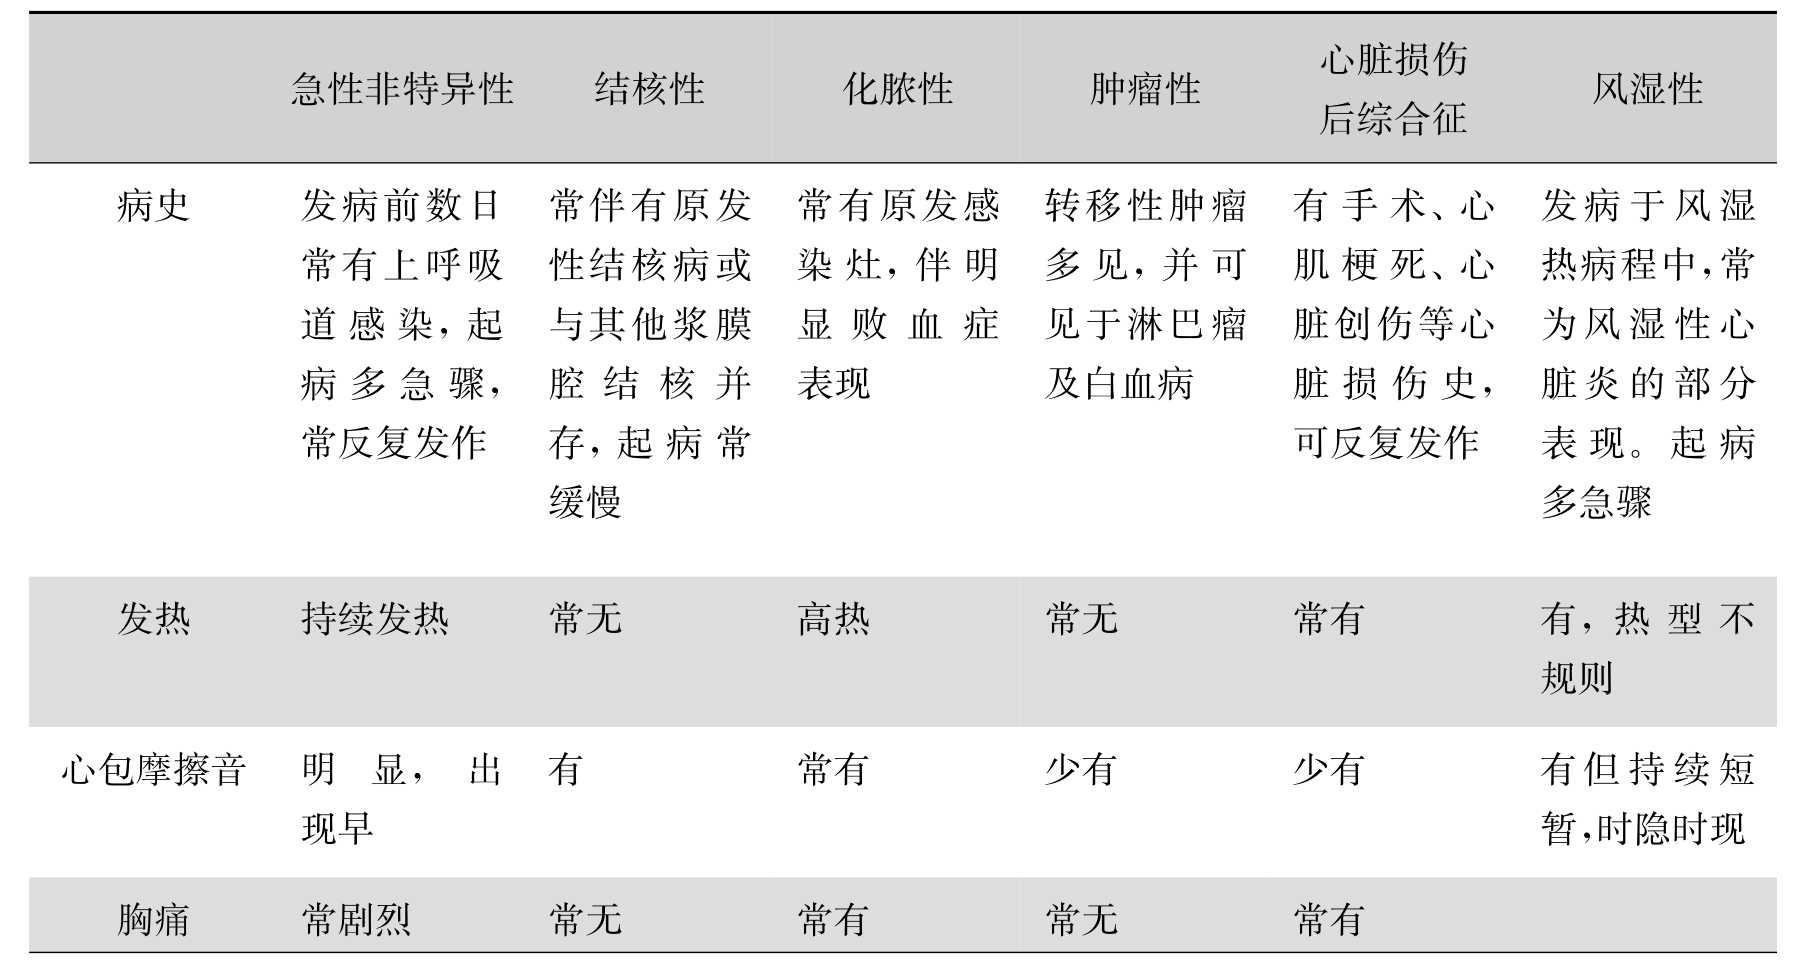
\includegraphics[width=5.96875in,height=3.21875in]{./images/Image00111.jpg}
%续表
\begin{longtable}{c}
  \caption{几种心包炎的鉴别诊断}
  \label{tabhello}
  \endfirsthead
  \caption[]{几种心包炎的鉴别诊断}
  \endhead
  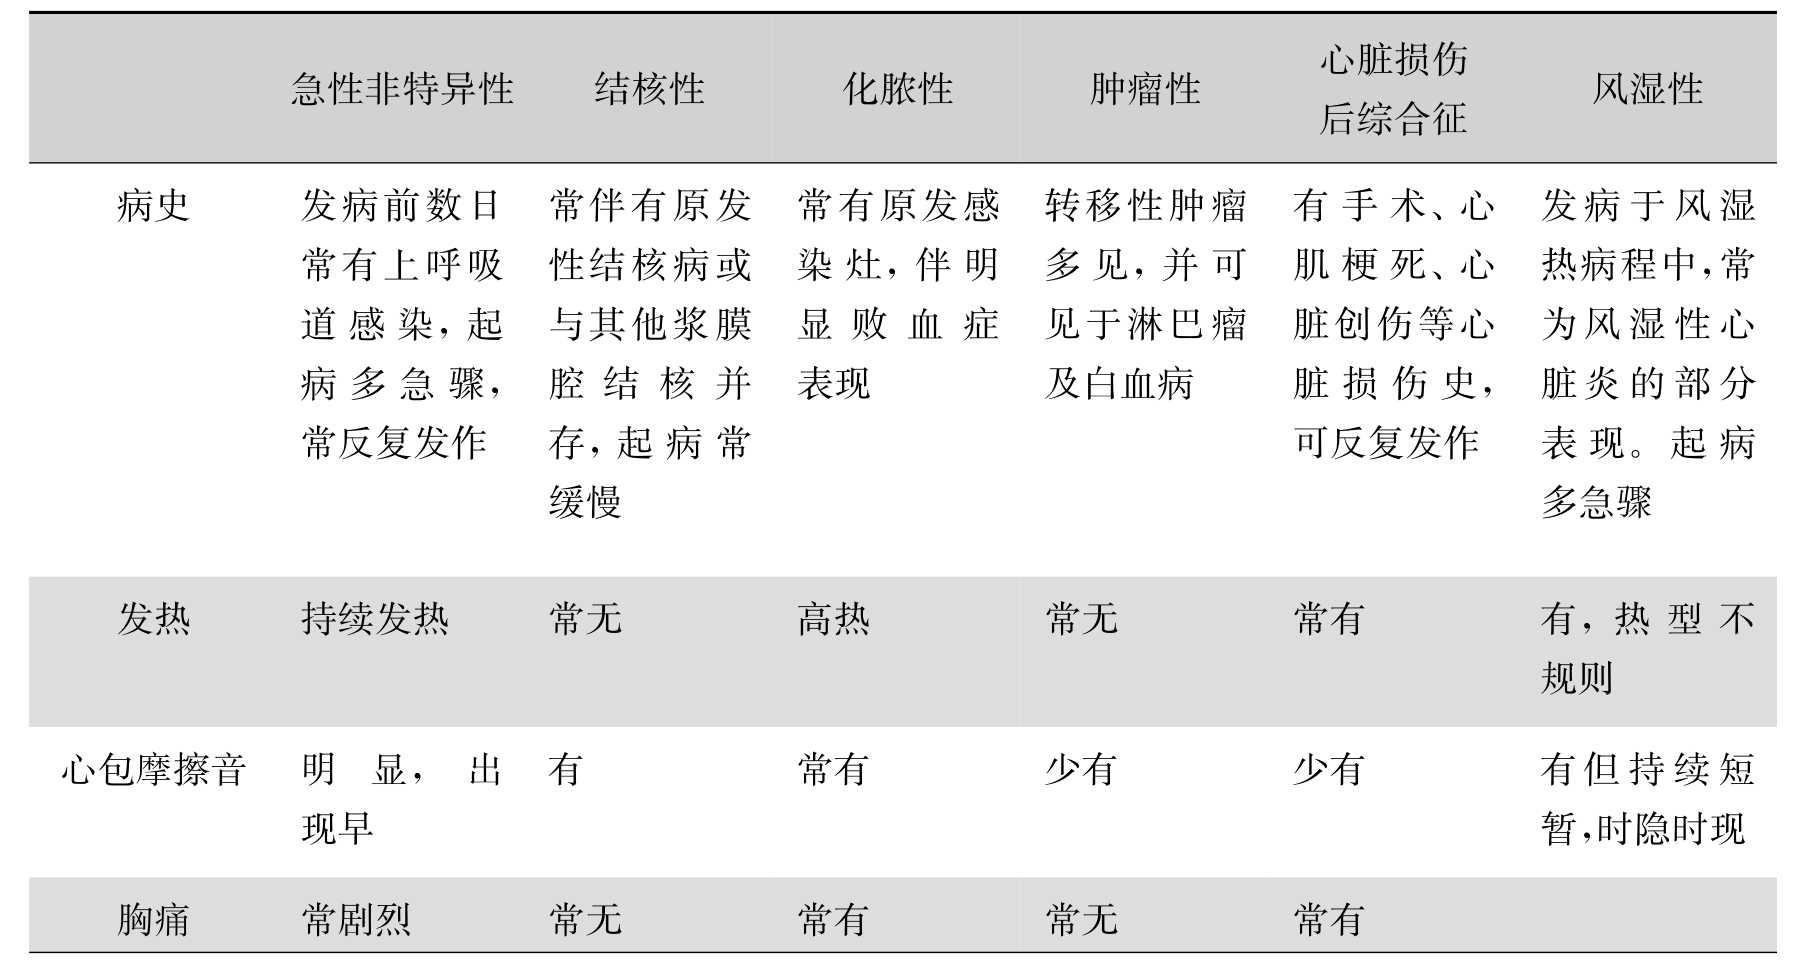
\includegraphics[width=\textwidth,height=\textheight,keepaspectratio]{./images/Image00111.jpg}\\
  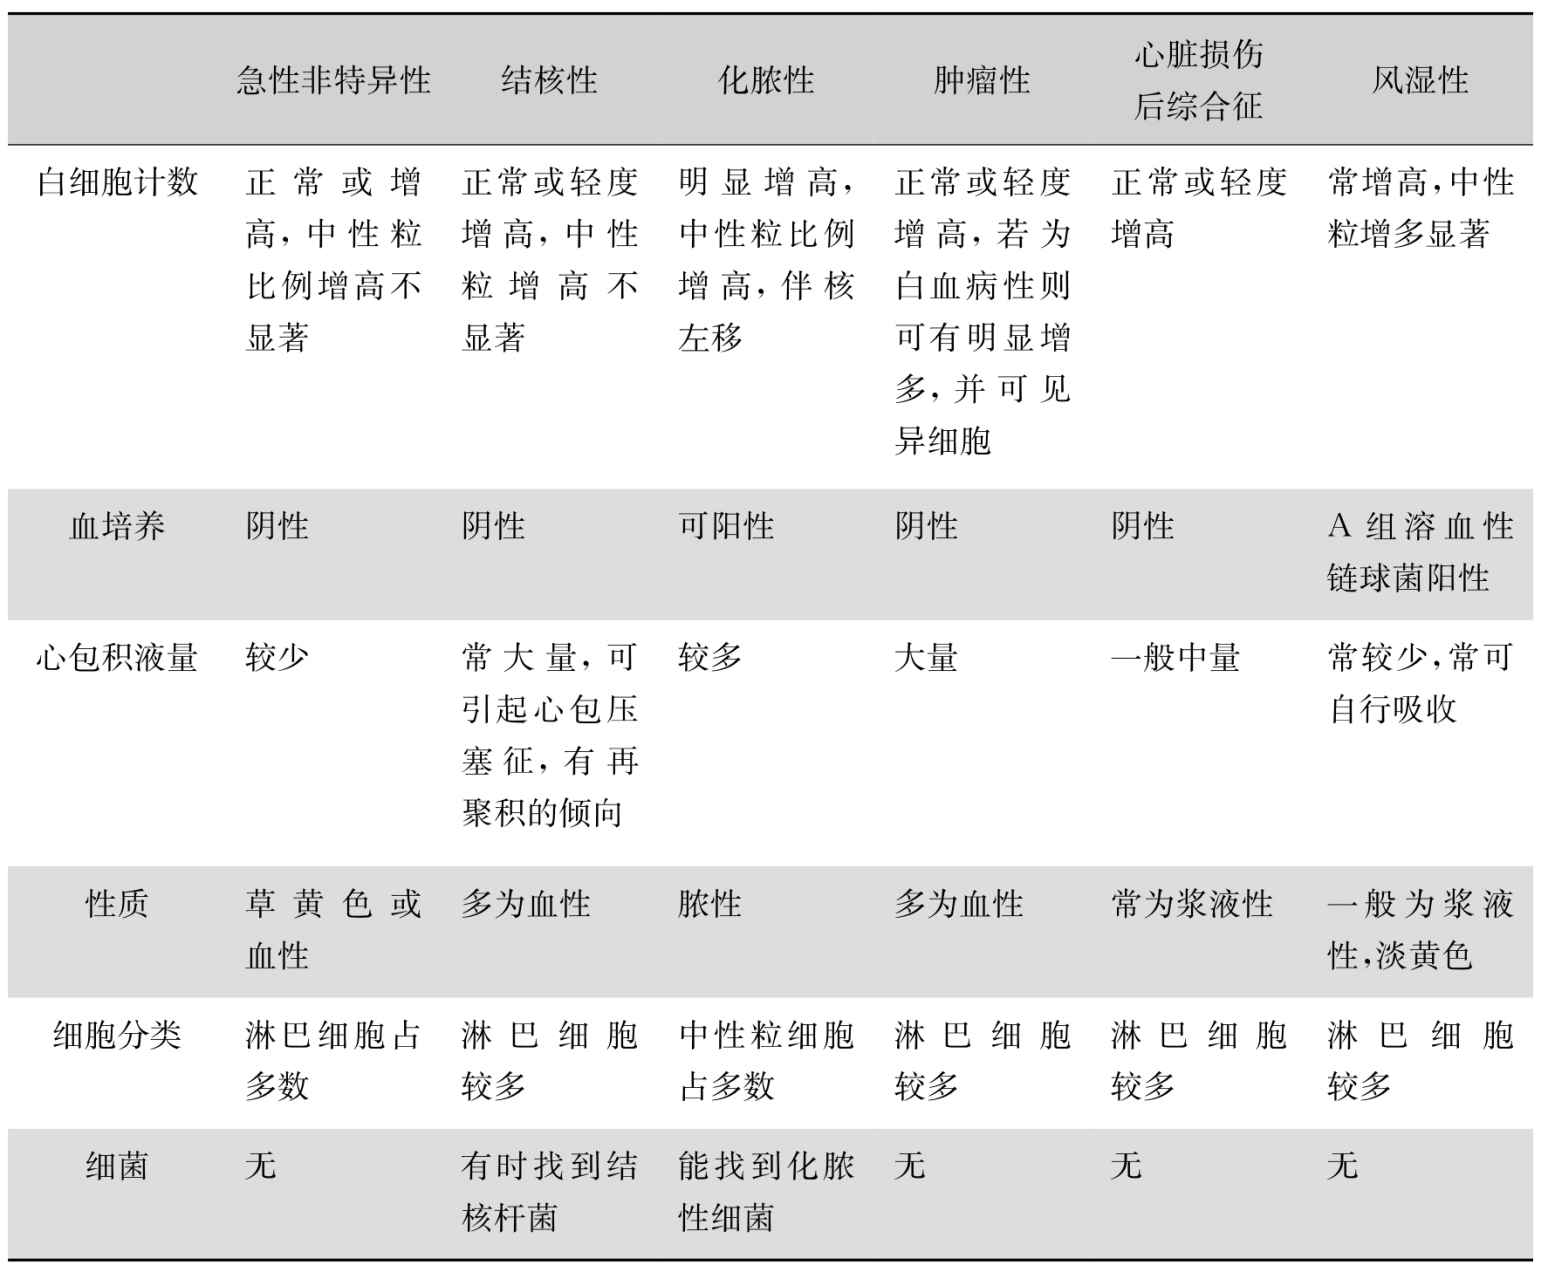
\includegraphics[width=\textwidth,height=\textheight,keepaspectratio]{./images/Image00112.jpg}
\end{longtable}

%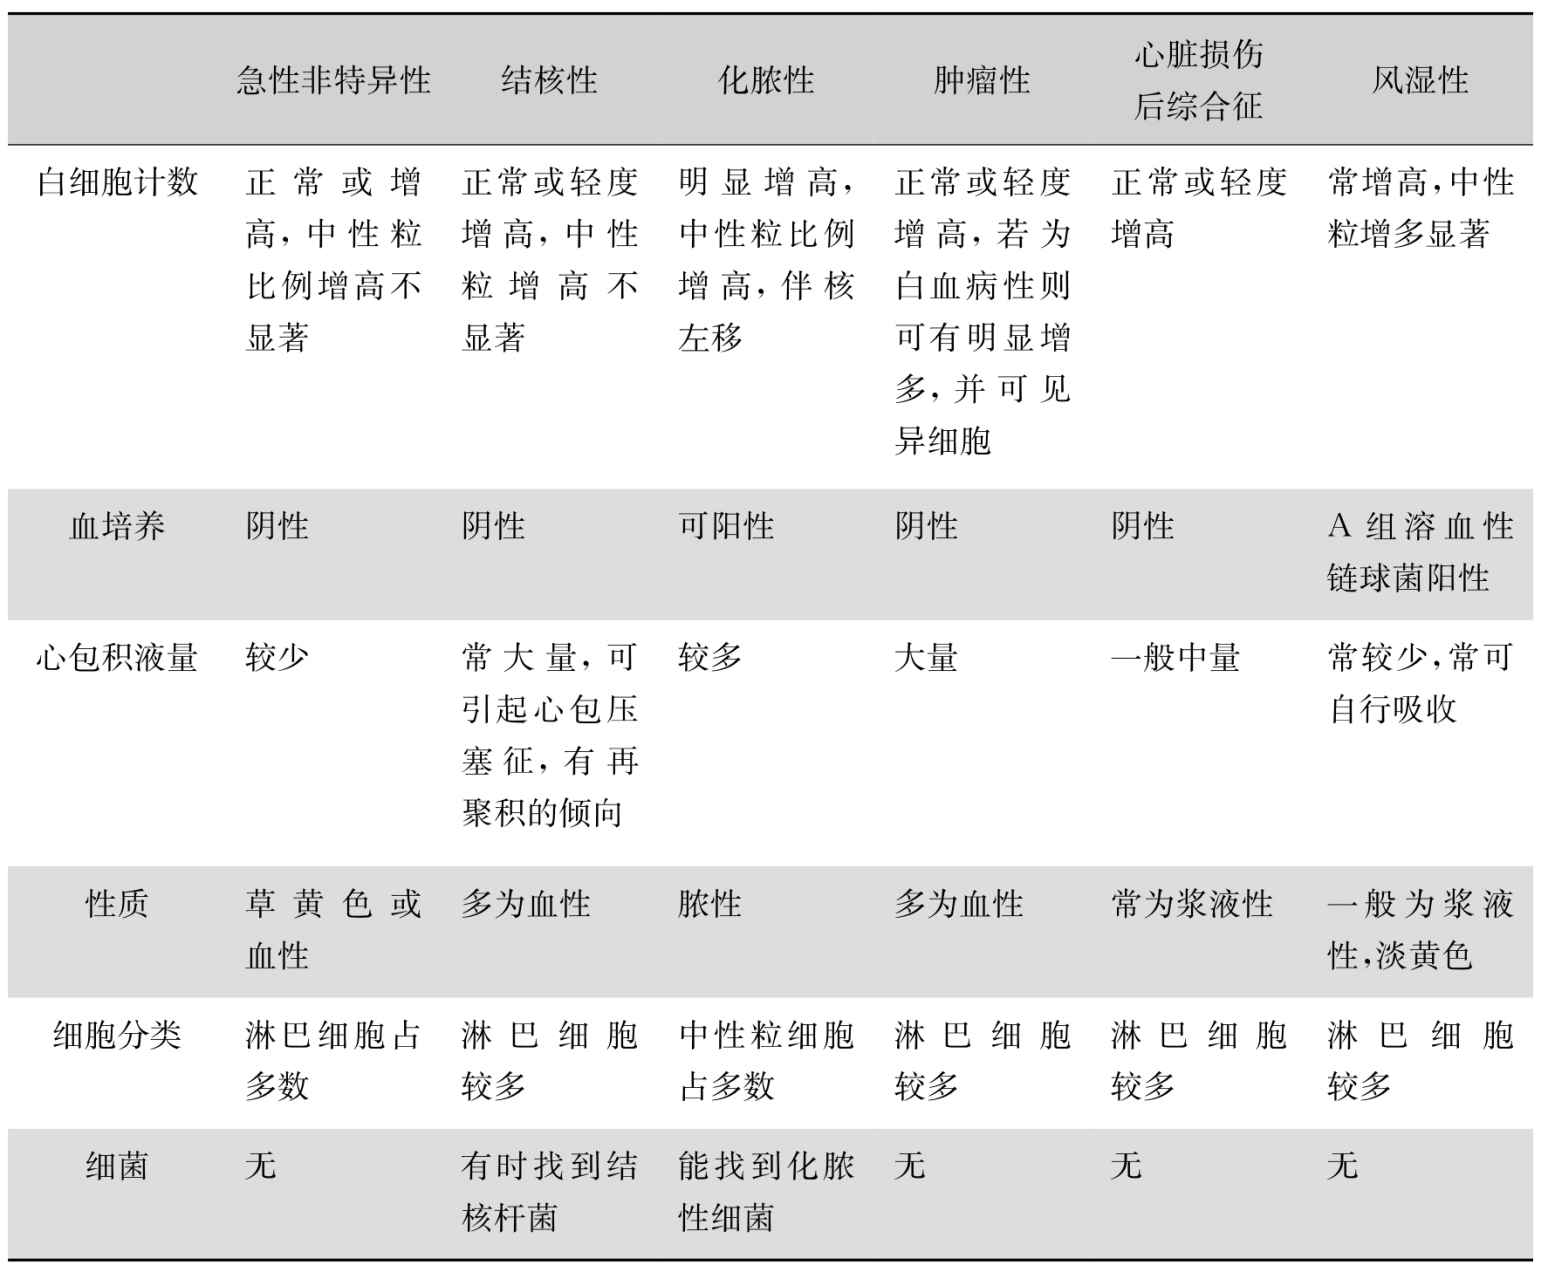
\includegraphics[width=5.90625in,height=4.875in]{./images/Image00112.jpg}

\protect\hypertarget{text00147.html}{}{}

\section{参考文献}

1.杨成悌,等.国内2999例心包炎病因分析.临床荟萃,2002,17(8):450-451

2.李海帆,等.胆固醇性心包炎二例.中华心血管病杂志,2003,31(7):527

3.马建新,等.放射性心包炎24例分析.中华放射肿瘤学杂志,2003,12:56

4.赵仙先,等.胸闷、胸痛、腹胀、心包积液.中华心血管病杂志,2004,32(6):561-563

5.李青,等.以心包炎为首发症状的带状疱疹一例.中华心血管病杂志,2003,31(10):781

6.刘永太,等.42例白塞病心脏损害患者的临床特点分析.中华内科杂志,2007,46(7):537-540

7.郝孝君,等.亚急性甲状腺炎合并心包积液一例.中华老年病学杂志,2002,21(2):92

8.刘平,等.氨氯地平致心包积液、胸腔积液、腹水及全身水肿一例.中华老年医学杂志,2002,21(6):466

9.喻磊,等.24例原发性心脏及心包恶性肿瘤的诊断与治疗.中华肿瘤杂志,2009,31(3):230-232

10.吉恒东,等.类风湿关节炎心脏损害36例临床分析.中华全科医学杂志,2011,9(3):403-404

\protect\hypertarget{text00148.html}{}{}

